Many approaches of vision systems employing region segmentation \cite{fast_segmentation_Mitra} \cite{fuzzy_segmentation} by color were developed lately. Real-time color based algorithms can be implemented by hardware, but this document describes a fast and non-specific-platform software to deal with it.  \\

\begin{figure}[th]
	\centering
	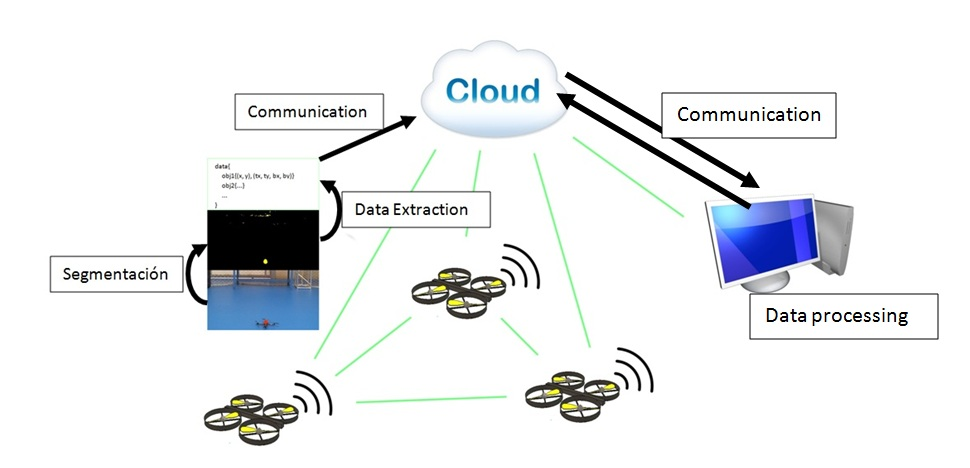
\includegraphics[width=\linewidth]{../Images/c1/schema_example_tags}
	\caption{}
	\label{fig:schema_example}
\end{figure}

The software is composed in three parts: Fist one deal with the image, extracting the 2D-objects, this step is called Color Image Segmentation \cite{JamesBruce_CMU_SEG} (or Color Cluster Segmentation: \textbf{CCS} in future mentions); The second one, receive the 2D-object of the previous step and math the objects between two cameras; Afterward the Extended Kalman Filter \cite{GabrielTerejanu_EKF} (\textbf{EKF}), performing with geometric, return the 3D-objects. The last part of the software deal with the communication between both observers in order to arrange the information. Later in section 1.6, a larger explanation of the Software Architecture will be provided.


Previous to the explanation of every step of the algorithm, the following pseudo-code describe the execution of the process.

\begin{algorithm}[hp]
\caption{Tracking algorithm}\label{algorithm_pseudo}
	\begin{algorithmic}[1]
	\Procedure{MainProcess}{}
		\State \Call{setUpEKF}{$params$}
		\State \Call{open}{$camera$}
		\State $\textit{img}  \gets$ \Call{GetImage}{$camera$}
		\If{$\textit{img}$ is empty} 
			\State \Return false
		\EndIf
		
		\State $\textit{objects} \gets$ \Call{Segmentation}{$img$}
		\If{size of $\textit{objects}$} 
			\State \Return false;
		\EndIf
		
		\State $\textit{state} \gets$ \Call{Tracking}{$objects$}
	\EndProcedure
	
	% --------------------------------------------------------------------------
	\Procedure{GetImage}{$VideoSource$}
		\If{$VideoSource$ is open}
			\State $image \gets VideoSource$
			\Return $image$
		\Else $\;$
			\State \Return $Null$
		\EndIf
		
	\EndProcedure
	
	% --------------------------------------------------------------------------	
	\Procedure{Segmentation}{$Image$}
		\If{$Image$ is not HSV}
			\State \Call{convertToHSV}{$Image$}
		\EndIf
		\ForAll{$pixel$ in $Image$}
			\State $pixel \gets$ \Call{conversion}{$pixel$}
		\EndFor
			\State \Return \Call{gatherObjects}{$Image$}
	\EndProcedure
	
	% --------------------------------------------------------------------------		
	\Procedure{Tracking}{$Object$}
		\State $matchedObj \gets$ \Call{Matching}{$Objects$} 
		\If{$matchedObj$ is empty}
			\State \Return $Null$
		\EndIf
		\State $state \gets$ \Call{stepEKF}{matchedObj}
		\State \Return $state$
	\EndProcedure
	
	% --------------------------------------------------------------------------	
	\end{algorithmic}
\end{algorithm}